
% xetex expected
\documentclass[xetex,professionalfont]{beamer}

% we want math
\usepackage{amsmath}

% fixes and extensions to amsmath
\usepackage{mathtools}

% additional math symbols
\usepackage{amssymb}

% good-looking fractions in text via \sfrac
\usepackage{xfrac}

% fix spaces after custom commands (see below for examples)
\usepackage{xspace}

% minted allows for fancy syntax highlighting (requires python with pygments)
% usage:
%   \begin{minted}{python}
%   codeb
%   \end{minted}
\usepackage{minted}

% better looking tables
% usage:
%   begin with a \toprule, write a single row of column headings,
%   then add \midrule and after the columns of data we finish with \bottomrule
% example:
%   \begin{tabular}{llr} \toprule
%   Animal & Description & Price \midrule
%   cat & foo & 10 \\
%   dog & bar & 20 \\ \bottomrule
%   \end{tabular}
% note that good tables generally neither have vertical rules nor double rules
\usepackage{booktabs}

% system font support (requires xetex or luatex)
\usepackage{fontspec}
\setmonofont[Scale=0.7]{Cousine} % part of ttf-chromeos fonts on Arch

% multi-language quotes for babel
\usepackage{csquotes}

% easy way to include copyright information
\usepackage{copyrightbox}

% better bibliographies
\usepackage[backend=biber,style=authoryear]{biblatex}

% language support (english,ngerman)
\usepackage[english]{babel}

% minted screws up line spacings ...
\usepackage{setspace}
\usepackage{enumitem}

% -----------------------------------------------------------------------------

% specify PDF metadata
\hypersetup{pdftitle={CVSP VO - Languages and Libraries},pdfsubject={},pdfauthor={Christopher Pramerdorfer}}

% copyright font style
\makeatletter\renewcommand{\CRB@setcopyrightfont}{\tiny\color{lightgray}}

% add bib file
\addbibresource{literature.bib}

% use tuwcvl beamer theme
\usetheme{tuwcvl}

% add some space between lines
\setstretch{1.4}

% but not for minted environments
\AtBeginEnvironment{minted}{\singlespacing}

% fix itemize

\setlist{nolistsep}
\setitemize{itemsep=-1mm,label=\usebeamerfont*{itemize item}%
  \usebeamercolor[fg]{itemize item}
  \usebeamertemplate{itemize item}}

% -----------------------------------------------------------------------------

% common english abbreviations
\newcommand{\ie}{\mbox{i.e.}\xspace} % i.e.
\newcommand{\eg}{\mbox{e.g.}\xspace} % e.g.

% math - argmin and argmax
\DeclareMathOperator*{\argmin}{arg\,min}
\DeclareMathOperator*{\argmax}{arg\,max}

% shortcuts for number ranges
\newcommand{\NN}{\mathbb{N}}
\newcommand{\ZZ}{\mathbb{Z}}
\newcommand{\QQ}{\mathbb{Q}}
\newcommand{\RR}{\mathbb{R}}

% bold vectors
\renewcommand{\vec}[1]{\ensuremath{\mathbf{#1}}}

% vector shortcuts
\newcommand{\va}{\vec{a}}
\newcommand{\vb}{\vec{b}}
\newcommand{\vc}{\vec{c}}
\newcommand{\ve}{\vec{e}}
\newcommand{\vr}{\vec{r}}
\newcommand{\vs}{\vec{s}}
\newcommand{\vt}{\vec{t}}
\newcommand{\vu}{\vec{u}}
\newcommand{\vv}{\vec{v}}
\newcommand{\vw}{\vec{w}}
\newcommand{\vx}{\vec{x}}
\newcommand{\vy}{\vec{y}}
\newcommand{\vz}{\vec{z}}

% highlight
\newcommand{\highlight}[1]{\textcolor{tuwcvl_inf_red}{\textbf{#1}}}

% -----------------------------------------------------------------------------

\title{Computer Vision Systems Programming VO}
\subtitle{Programming Languages and Libraries}
\author{Christopher Pramerdorfer}
\institute{Computer Vision Lab, Vienna University of Technology}

\begin{document}

% -----------------------------------------------------------------------------

\begin{frame}
\maketitle
\end{frame}

% -----------------------------------------------------------------------------

\begin{frame}
\frametitle{Topics}

Characteristics of Computer Vision (CV) programming
\begin{itemize}
	\item Implications on programming language choice
\end{itemize}

\medskip
Which language is the best?

\medskip
Overview of popular languages and libraries
\begin{itemize}
	\item Matlab
	\item Python
	\item C++
\end{itemize}

\medskip
Suggestions on language selection

\end{frame}

% -----------------------------------------------------------------------------

\begin{frame}
\frametitle{Characteristics of CV Programming}
\framesubtitle{Image Processing}

We often start with Image Processing (IP)
\begin{itemize}
	\item Resampling, normalization, color conversion
	\item Feature extraction
\end{itemize}

\medskip
Involves operations on arrays / matrices

\medskip
Many IP operations are local and sequential
\begin{itemize}
	\item Favors languages with fast random access to pixels % "don't code loops in matlab" should sound familiar
\end{itemize}

\end{frame}

% -----------------------------------------------------------------------------

\begin{frame}
\frametitle{Characteristics of CV Programming}
\framesubtitle{Many IP Operations Are Local and Sequential}

Image resampling is done independently for each pixel\\ % in the target image
Involves some form of local interpolation

\medskip
\begin{center}
	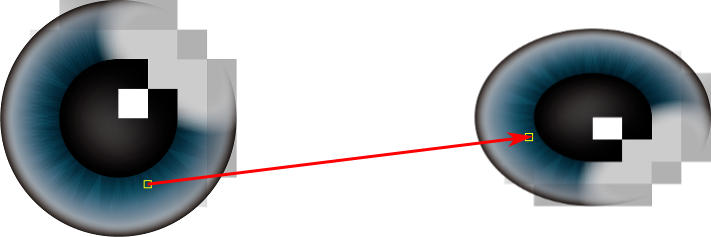
\includegraphics[width=8cm]{figures/resampling.png}
\end{center}

\end{frame}

% -----------------------------------------------------------------------------

\begin{frame}
\frametitle{Characteristics of CV Programming}
\framesubtitle{Many IP Operations Are Local and Sequential}

Local neighborhood operations such as linear filtering:
\[
 f'(x,y)=\sum_{i,j}f(x+i,y+j)\,h(i,j)
\]

\medskip
\begin{center}
	\copyrightbox[b]
	{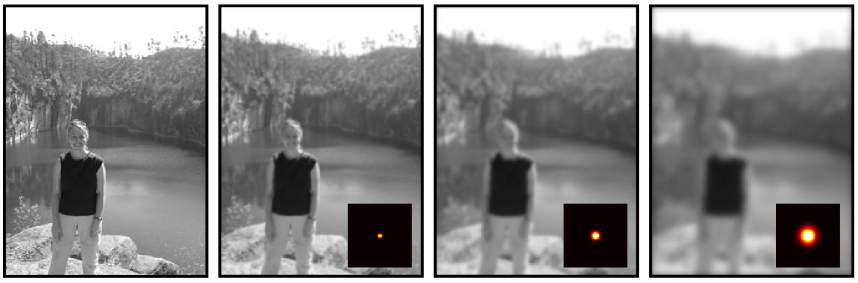
\includegraphics[width=8cm]{figures/blur-example.png}}
	{\centering Image from \cite{prince12}}
\end{center}

\end{frame}

% -----------------------------------------------------------------------------

\begin{frame}
\frametitle{Characteristics of CV Programming}
\framesubtitle{Numerical Computing}

More generally, CV programming is all about numbers

\medskip
Often, there are many of them
\begin{itemize}
	\item BD stream: $\sim$ 50 million/sec % 1920*1080*24
	\item Large optimization problems
\end{itemize}

\medskip
Some languages are better at crunching numbers than others
\begin{itemize}
	\item Faster, more memory-efficient
\end{itemize}

\end{frame}

% -----------------------------------------------------------------------------

\begin{frame}
\frametitle{Characteristics of CV Programming}
\framesubtitle{Does Speed and Efficiency Matter?}

It depends!
\begin{itemize}
	\item Researchers often don't care % but sometimes they do - for example training convnets can take weeks even on GPUs - would not be feasible without heavy software optimization
	\item Companies usually do % run more analysis channels on a the same machine = money saved
	\item Sometimes there are hard constraints (cars, space missions)
\end{itemize}

\medskip
\begin{center}
	\copyrightbox[b]
	{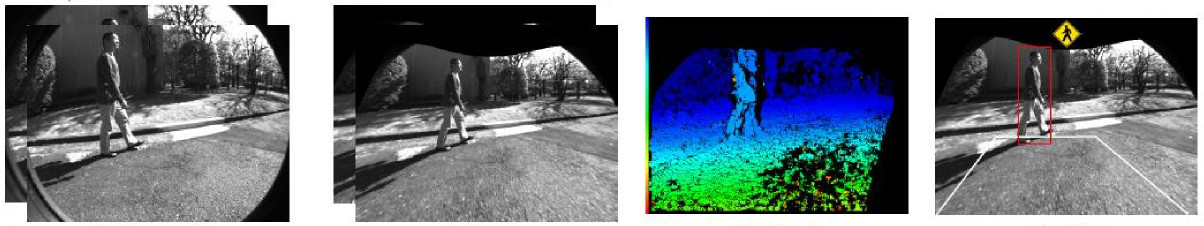
\includegraphics[width=10cm]{figures/car-pedestrian.jpg}}
	{\centering Image by Ryuzo Okada, Toshiba}
\end{center}

\end{frame}

% -----------------------------------------------------------------------------

\begin{frame}
\frametitle{Characteristics of CV Programming}
\framesubtitle{Does Speed and Efficiency Matter?}

Design choices can have a bigger impact than language
\begin{itemize}
	\item Use appropriate data structures
	\item Utilize multiple CPU cores, GPUs
\end{itemize}

\medskip
Language bottlenecks can be avoided by switching language
\begin{itemize}
	\item Interpreted languages are slow \enquote{at the pixel level} % loops over pixels
	\item Implement such parts in C, call from Matlab, Python
	\item Use higher-level functions (\texttt{mean}, \texttt{imfilter}) % that are themselves written in c
\end{itemize}

\end{frame}

% -----------------------------------------------------------------------------

\begin{frame}
\frametitle{Choosing a Programming Language}
\framesubtitle{Other Factors}

There are other important factors in language selection
\begin{itemize}
	\item Ease of development (language features, libraries, IDEs)
	\item OS and platform support % does it run on all OS? does it run on ARM like the odroid shown below?
	\item License fees % matlab is 2000 euros as of oct 2014
\end{itemize}

\medskip
\begin{center}
	\copyrightbox[b]
	{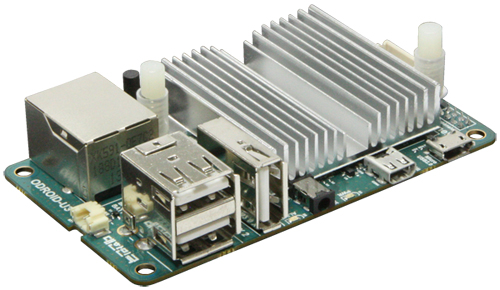
\includegraphics[width=4.5cm]{figures/odroid-u3.jpg}}
	{\centering Image from \url{pixhawk.org}}
\end{center}

\end{frame}

% -----------------------------------------------------------------------------

\begin{frame}
\frametitle{Choosing a Programming Language}

So there is no \textit{best} language, it depends
\begin{itemize}
	\item On the task at hand % pedestrian detection ...
	\item On the operating conditions % for a paper? speed usually not important / for use in cars? different story!
\end{itemize}

\medskip
Let's take a look at some popular languages and libraries

\end{frame}

% -----------------------------------------------------------------------------

\begin{frame}
\frametitle{Popular CV Programming Languages}

\begin{figure}
\centering
{\copyrightbox[b]
	{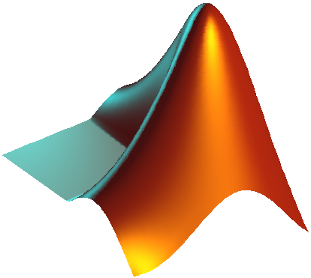
\includegraphics[width=2.8cm]{figures/matlab-logo.png}}
	{\centering Image from \url{matworks.de}}}\quad
{\copyrightbox[b]
	{
\includegraphics[width=4.5cm]{figures/python-logo.png}}
	{\centering Image from \url{python.org}}}\quad
{\copyrightbox[b]
	{
\includegraphics[width=2.2cm]{figures/cpp-logo.jpg}}
	{\centering Image from \url{cplusplus.se}}}
\end{figure}

\end{frame}

% -----------------------------------------------------------------------------

\begin{frame}
\frametitle{Popular CV Programming Languages}
\framesubtitle{Matlab}

\begin{columns}
\column{0.65\textwidth}

Numerical computing environment \\
Commercial software (student licenses)\\
Widely used in academics \\
Used in many courses at TU Wien

\column{0.25\textwidth}

\begin{center}
{\copyrightbox[b]
	{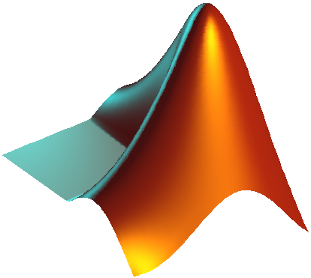
\includegraphics[width=2.3cm]{figures/matlab-logo.png}}
	{\centering Image from \url{matworks.de}}}
\end{center}

\end{columns}

\end{frame}

% -----------------------------------------------------------------------------

\begin{frame}
\frametitle{Popular CV Programming Languages}
\framesubtitle{Matlab}

Pros
\begin{itemize}
	\item Easy to learn and use
	\item Many high-quality toolboxes
\end{itemize}

\medskip
Cons
\begin{itemize}
	\item Not as fast/efficient from scratch as C++ % code is fast if vectorized, but that can be tedious work
	\item Commercial licenses are expensive
	\item Less suitable for general-purpose programming
\end{itemize}

\end{frame}

% -----------------------------------------------------------------------------

\begin{frame}
\frametitle{Popular CV Programming Languages}
\framesubtitle{Python}

\begin{columns}
\column{0.65\textwidth}

General-purpose programming language \\
Free and open source\\ % This applies to the Cython reference implementation
No IP/CV functionality by default \\
But great open-source libraries

\column{0.25\textwidth}

\begin{center}
{\copyrightbox[b]
	{
\includegraphics[width=2.6cm]{figures/python-logo.png}}
	{\centering Image from \url{python.org}}}
\end{center}

\end{columns}

\end{frame}

% -----------------------------------------------------------------------------

\begin{frame}
\frametitle{Popular CV Programming Languages}
\framesubtitle{Python}

Pros
\begin{itemize}
	\item Easy to learn and use
	\item Extensive standard library
	\item Free and open source
\end{itemize}

\medskip
Cons
\begin{itemize}
	\item Not as integrated as Matlab
	\item Not as fast/efficient from scratch as C++ % code is fast if vectorized, but that can be tedious work
\end{itemize}

\end{frame}

% -----------------------------------------------------------------------------

\begin{frame}
\frametitle{Popular CV Programming Languages}
\framesubtitle{Python -- NumPy}

\begin{columns}
\column{0.65\textwidth}

Fundamental numerical computing library

\medskip
Arrays and matrices\\
Linear algebra\\
Matrix decompositions\\ % svd, qr, cholesky
Fourier analysis

\column{0.25\textwidth}

\begin{center}
{\copyrightbox[b]
	{
\includegraphics[width=2.6cm]{figures/numpy-logo.png}}
	{\centering Image from \url{github.com/numpy}}}
\end{center}

\end{columns}

\end{frame}

% -----------------------------------------------------------------------------

\begin{frame}
\frametitle{Popular CV Programming Languages}
\framesubtitle{Python -- SciPy}

\begin{columns}
\column{0.65\textwidth}

Family of scientific computing packages % like numpy, matplotlib

\medskip
Optimization\\
Image processing\\ % linear filtering, morphology, distance transform, segmentation
Statistics \& density estimation

\column{0.25\textwidth}

\begin{center}
{\copyrightbox[b]
	{
\includegraphics[width=2.3cm]{figures/scipy-logo.png}}
	{\centering Image from \url{scipy.org}}}
\end{center}

\end{columns}

\end{frame}

% -----------------------------------------------------------------------------

\begin{frame}
\frametitle{Popular CV Programming Languages}
\framesubtitle{Python -- scikit-image}

\begin{columns}
\column{0.65\textwidth}

Image processing library

\medskip
Image transforms\\
Image filtering\\
Feature extraction\\
Segmentation % e.g. graphcut, watershed

\column{0.25\textwidth}

\begin{center}
{\copyrightbox[b]
	{
\includegraphics[width=2.6cm]{figures/ski-logo.png}}
	{\centering Image from \url{scikit-image.org}}}
\end{center}

\end{columns}

\end{frame}

% -----------------------------------------------------------------------------

\begin{frame}
\frametitle{Popular CV Programming Languages}
\framesubtitle{Python -- scikit-learn}

\begin{columns}
\column{0.65\textwidth}

Comprehensive machine learning library

\medskip
Classification\\
Regression\\
Clustering\\
Dimensionality reduction

\column{0.25\textwidth}

\begin{center}
{\copyrightbox[b]
	{
\includegraphics[width=2.6cm]{figures/skl-logo.png}}
	{\centering Image from \url{goodfind.jp}}}
\end{center}

\end{columns}

\end{frame}

% -----------------------------------------------------------------------------

\begin{frame}
\frametitle{Popular CV Programming Languages}
\framesubtitle{Python -- Keras}

\begin{columns}
\column{0.65\textwidth}

Deep learning library

\medskip
Multilayer Perceptrons \\
Convolutional Neural Networks \\
Recurrent Neural Networks \\
CPU and GPU using CUDA

\column{0.25\textwidth}

\begin{center}
{\copyrightbox[b]
	{
\includegraphics[width=2.6cm]{figures/keras-logo.jpg}}
	{\centering Image from \url{keras.io}}}
\end{center}

\end{columns}

\end{frame}

% -----------------------------------------------------------------------------

\begin{frame}
\frametitle{Popular CV Programming Languages}
\framesubtitle{Python -- matplotlib}

\begin{columns}
\column{0.65\textwidth}

Graph plotting library

\medskip
Surface, wireframe, scatter, bar plots\\
Matlab-like syntax

\column{0.25\textwidth}

\begin{center}
{\copyrightbox[b]
	{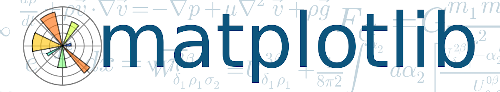
\includegraphics[width=2.6cm]{figures/matplotlib-logo.png}}
	{\centering Image from \url{matplotlib.org}}}
\end{center}

\end{columns}

\end{frame}

% -----------------------------------------------------------------------------

\begin{frame}
\frametitle{Popular CV Programming Languages}
\framesubtitle{C++}

\begin{columns}
\column{0.65\textwidth}

General-purpose programming language\\
Focus on performance and efficiency\\
No IP/CV functionality by default\\
But great open-source libraries

\column{0.25\textwidth}

\begin{center}
{\copyrightbox[b]
	{
\includegraphics[width=2.3cm]{figures/cpp-logo.jpg}}
	{\centering Image from \url{cplusplus.se}}}
\end{center}

\end{columns}

\end{frame}

% -----------------------------------------------------------------------------

\begin{frame}
\frametitle{Popular CV Programming Languages}
\framesubtitle{C++}

Pros
\begin{itemize}
	\item Fast and memory-efficient
	\item Free and open source
\end{itemize}

\medskip
Cons
\begin{itemize}
	\item Harder to learn and master
	\item Slower and less convenient to code
\end{itemize}

\end{frame}

% -----------------------------------------------------------------------------

\begin{frame}
\frametitle{Popular CV Programming Languages}
\framesubtitle{C++ -- OpenCV}

\begin{columns}
\column{0.65\textwidth}

Comprehensive IP/CV library\\
Designed for real-time applications

\medskip
Matrices and linear algebra\\
Image transforms and filtering\\
Feature extraction and matching\\
Stereo, structure from motion\\
Machine learning % boosting, trees, em, nn, svms, forests

\medskip
Matlab and Python bindings available

\column{0.25\textwidth}

\begin{center}
{\copyrightbox[b]
	{
\includegraphics[width=2.3cm]{figures/opencv-logo.png}}
	{\centering Image from \url{opencv.org}}}
\end{center}

\end{columns}

\end{frame}

% -----------------------------------------------------------------------------

\begin{frame}
\frametitle{Popular CV Programming Languages}
\framesubtitle{C++ -- Caffe}

Deep learning library

\medskip
Multilayer Perceptrons \\
Convolutional Neural Networks \\
CPU and GPU using CUDA

\medskip
Trained models available (model zoo)\\
Used by e.g.\ Nvidia, Google

\medskip
Matlab and Python bindings available

\end{frame}

% -----------------------------------------------------------------------------

\begin{frame}
\frametitle{Popular CV Programming Languages}
\framesubtitle{C++ -- MathGL}

\begin{columns}
\column{0.65\textwidth}

Graph plotting library

\medskip
Surface, wireframe, scatter, bar plots

\column{0.25\textwidth}

\begin{center}
{\copyrightbox[b]
	{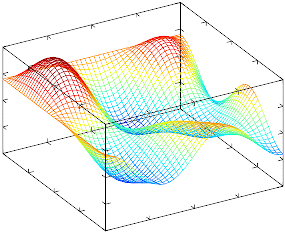
\includegraphics[width=2.6cm]{figures/mathgl-mesh.png}}
	{\centering Image from \url{mathgl.sourceforge.net}}}
\end{center}

\end{columns}

\end{frame}

% -----------------------------------------------------------------------------

\begin{frame}
\frametitle{Popular CV Programming Languages}
\framesubtitle{Remarks}

Comparable functionality
\begin{itemize}
	\item Libraries for most CV tasks available
	\item This applies to other languages as well
\end{itemize}

\medskip
Many libraries have language bindings

\end{frame}

% -----------------------------------------------------------------------------

\begin{frame}
\frametitle{Code Comparison}

Task is to load, blur, show, and save an image

\end{frame}

% -----------------------------------------------------------------------------

\begin{frame}[fragile]
\frametitle{Code Comparison}
\framesubtitle{Matlab}

\begin{minted}{matlab}
img = imread('image.png'); % read
kernel = fspecial('gaussian', [5 5]); % blur
blur = imfilter(img, kernel); % blur
imshow(blur); % display
pause(5); % wait
imwrite(blur, 'blur.png'); % save
\end{minted}

\end{frame}

% -----------------------------------------------------------------------------

\begin{frame}[fragile]
\frametitle{Code Comparison}
\framesubtitle{Python with scikit-image}

\begin{minted}{python}
img = skimage.io.imread('image.png') # read
blur = skimage.filter.gaussian_filter(img, sigma=1.7) # blur
skimage.io.imshow(blur) # display
skimage.io.show() # wait
skimage.io.imsave('blur.png', blur) # save
\end{minted}

\end{frame}

% -----------------------------------------------------------------------------

\begin{frame}[fragile]
\frametitle{Code Comparison}
\framesubtitle{C++ with OpenCV}

\begin{minted}{cpp}
cv::Mat img = cv::imread("image.png"); // read
cv::Mat blur; // blur
cv::GaussianBlur(img, blur, cv::Size(5, 5), 0); // blur
cv::imshow("blur", blur); // display
cv::waitKey(0); // wait
cv::imwrite("blur.png", blur); // save
\end{minted}

\end{frame}

% -----------------------------------------------------------------------------

\begin{frame}
\frametitle{Code Comparison}

Similar programming effort in the example case

\medskip
For many larger CV tasks
\begin{itemize}
	\item Matlab requires least effort
	\item Closely followed by Python
	\item Not so closely followed by C++
\end{itemize}

\medskip
Depends on the problem of course
\begin{itemize}
	\item Libraries available?
\end{itemize}

\end{frame}

% -----------------------------------------------------------------------------

\begin{frame}
\frametitle{Language Comparison}

In summary, the discussed languages
\begin{itemize}
	\item Differ in terms of execution speed and memory-efficiency
	\item Provide comparable CV programming functionality via libraries
	\item Differ in ease of development, licensing fees
\end{itemize}

\medskip
So, to conclude
\begin{itemize}
	\item There is no best CV language
	\item Different tasks favor different languages
\end{itemize}

\end{frame}

% -----------------------------------------------------------------------------

\begin{frame}
\frametitle{Suggestions on Language Selection}

Know the strengths and weaknesses of different languages

\medskip
Be proficient in more than one language
\begin{itemize}
	\item Allows you to select appropriate language for task at hand
	\item E.g.\ prototype in Matlab/Python, ship in C++
\end{itemize}

\medskip
Learn C++
\begin{itemize}
	\item Modern C++ is not a bad language if used correctly
	\item Some real-time applications require its speed and efficiency
	\item Many companies use it
\end{itemize}

\end{frame}

% -----------------------------------------------------------------------------

\begin{frame}
\frametitle{Bibliography}

\printbibliography

\end{frame}

\end{document}
